%% BioMed_Central_Tex_Template_v1.06
%%                                      %
%  bmc_article.tex            ver: 1.06 %
%                                       %

%%IMPORTANT: do not delete the first line of this template
%%It must be present to enable the BMC Submission system to
%%recognise this template!!

%%%%%%%%%%%%%%%%%%%%%%%%%%%%%%%%%%%%%%%%%
%%                                     %%
%%  LaTeX template for BioMed Central  %%
%%     journal article submissions     %%
%%                                     %%
%%          <8 June 2012>              %%
%%                                     %%
%%                                     %%
%%%%%%%%%%%%%%%%%%%%%%%%%%%%%%%%%%%%%%%%%

%%%%%%%%%%%%%%%%%%%%%%%%%%%%%%%%%%%%%%%%%%%%%%%%%%%%%%%%%%%%%%%%%%%%%
%%                                                                 %%
%% For instructions on how to fill out this Tex template           %%
%% document please refer to Readme.html and the instructions for   %%
%% authors page on the biomed central website                      %%
%% https://www.biomedcentral.com/getpublished                      %%
%%                                                                 %%
%% Please do not use \input{...} to include other tex files.       %%
%% Submit your LaTeX manuscript as one .tex document.              %%
%%                                                                 %%
%% All additional figures and files should be attached             %%
%% separately and not embedded in the \TeX\ document itself.       %%
%%                                                                 %%
%% BioMed Central currently use the MikTex distribution of         %%
%% TeX for Windows) of TeX and LaTeX.  This is available from      %%
%% https://miktex.org/                                             %%
%%                                                                 %%
%%%%%%%%%%%%%%%%%%%%%%%%%%%%%%%%%%%%%%%%%%%%%%%%%%%%%%%%%%%%%%%%%%%%%

%%% additional documentclass options:
%  [doublespacing]
%  [linenumbers]   - put the line numbers on margins

%%% loading packages, author definitions

\documentclass[twocolumn]{bmcart}% uncomment this for twocolumn layout
% and comment line below
%\documentclass{bmcart}

%%% Load packages
\usepackage{amsthm,amsmath}
%\RequirePackage[numbers]{natbib}
%\RequirePackage[authoryear]{natbib}% uncomment this for author-year bibliography
%\RequirePackage{hyperref}
\usepackage[utf8]{inputenc} %unicode support
%\usepackage[applemac]{inputenc} %applemac support if unicode package fails
%\usepackage[latin1]{inputenc} %UNIX support if unicode package fails


%%%%%%%%%%%%%%%%%%%%%%%%%%%%%%%%%%%%%%%%%%%%%%%%%
%%                                             %%
%%  If you wish to display your graphics for   %%
%%  your own use using includegraphic or       %%
%%  includegraphics, then comment out the      %%
%%  following two lines of code.               %%
%%  NB: These line *must* be included when     %%
%%  submitting to BMC.                         %%
%%  All figure files must be submitted as      %%
%%  separate graphics through the BMC          %%
%%  submission process, not included in the    %%
%%  submitted article.                         %%
%%                                             %%
%%%%%%%%%%%%%%%%%%%%%%%%%%%%%%%%%%%%%%%%%%%%%%%%%

%\def\includegraphic{}
%\def\includegraphics{}

%%% Put your definitions there:
\usepackage[ruled,vlined]{algorithm2e}
\usepackage{graphicx}
\usepackage{setspace}
\usepackage{url}

\startlocaldefs

%%%%%%%%%%%%%%%%%%%%%%%%%%%%%%%%%%%%%%%%%%%%%%%
%% Data inline
%%%%%%%%%%%%%%%%%%%%%%%%%%%%%%%%%%%%%%%%%%%%%%%

\newcommand{\dataInterRater}{0.94 (95\% CI: 0.93 – 0.95)}
\newcommand{\dataNumItus}{178}
\newcommand{\dataOverallAccuracy}{72.6\% (label propagation) versus 72.4\% (activity based)}
\newcommand{\dataCorrect}{12534}
\newcommand{\dataTotal}{17274}
\newcommand{\dataMcc}{0.72}
\newcommand{\dataTopMisclass}{1833}
\newcommand{\dataTopMisclassPercent}{38.7\%}
\newcommand{\dataAcc}{72.6\%}

\providecommand{\tightlist}{%
  \setlength{\itemsep}{0pt}\setlength{\parskip}{0pt}}
  
\endlocaldefs

%%% Begin ...
\begin{document}

%%% Start of article front matter
\begin{frontmatter}

\begin{fmbox}
\dochead{Research}

%%%%%%%%%%%%%%%%%%%%%%%%%%%%%%%%%%%%%%%%%%%%%%
%%                                          %%
%% Enter the title of your article here     %%
%%                                          %%
%%%%%%%%%%%%%%%%%%%%%%%%%%%%%%%%%%%%%%%%%%%%%%

\title{Algorithmic hospital catchment area estimation using label propagation}

%%%%%%%%%%%%%%%%%%%%%%%%%%%%%%%%%%%%%%%%%%%%%%
%%                                          %%
%% Enter the authors here                   %%
%%                                          %%
%% Specify information, if available,       %%
%% in the form:                             %%
%%   <key>={<id1>,<id2>}                    %%
%%   <key>=                                 %%
%% Comment or delete the keys which are     %%
%% not used. Repeat \author command as much %%
%% as required.                             %%
%%                                          %%
%%%%%%%%%%%%%%%%%%%%%%%%%%%%%%%%%%%%%%%%%%%%%%

\author[
  addressref={aff1,aff2},
  corref={aff1},
  email={rc538@exeter.ac.uk}
]{\inits{R.J.} \fnm{Robert J.} \snm{Challen}}
\author[
  addressref={aff3,aff4},
  email={g.griffith@bristol.ac.uk}
]{\inits{G.J.} \fnm{Gareth J.} \snm{Griffith}}
\author[
  addressref={aff5,aff6},
  email={lucas@ifisc.uib-csic.es}
]{\inits{L.} \fnm{Lucas} \snm{Lacasa}}
\author[
  addressref={aff1,aff7,aff8},
  email={k.tsaneva-atanasova@exeter.ac.uk}
]{\inits{K.} \fnm{Krasimira} \snm{Tsaneva-Atanasova}}


%%%%%%%%%%%%%%%%%%%%%%%%%%%%%%%%%%%%%%%%%%%%%%
%%                                          %%
%% Enter the authors' addresses here        %%
%%                                          %%
%% Repeat \address commands as much as      %%
%% required.                                %%
%%                                          %%
%%%%%%%%%%%%%%%%%%%%%%%%%%%%%%%%%%%%%%%%%%%%%%

\address[id=aff1]{% 
  \orgdiv{Hub for Quantitative Modelling in Healthcare},
  \orgname{University of Exeter},
  \city{Exeter},
  \cny{UK}.
}
\address[id=aff2]{% 
  \orgname{Somerset NHS Foundation Trust}, 
  \city{Taunton}, 
  \cny{UK}.
}
\address[id=aff3]{% 
  \orgdiv{Bristol Medical School, Population Health Sciences},
  \orgname{University of Bristol}, 
  \city{Bristol}, 
  \cny{UK}.
}
\address[id=aff4]{% 
  \orgdiv{Medical Research Council Integrative Epidemiology Unit}, 
  \orgname{University of Bristol}, 
  \city{Bristol}, 
  \cny{UK}.
}
\address[id=aff5]{% 
  \orgdiv{School of Mathematical Sciences}, 
  \orgname{Queen Mary University of London},
  \city{London}, 
  \cny{UK}
}
\address[id=aff6]{% 
  \orgdiv{Instituto de Física Interdisciplinar y Sistemas Complejos (IFISC)}
  \orgname{Universidad de las Islas Baleares, CSIC-UIB},
  \city{Palma de Mallorca}, 
  \cny{Spain}
}
\address[id=aff7]{% 
  \orgdiv{The Alan Turing Institute}, 
  \orgname{British Library},
  \city{London},
  \cny{UK}.
}
\address[id=aff8]{% 
  \orgdiv{Data Science Institute}, 
  \orgname{University of Exeter},
  \city{Exeter},
  \cny{UK}.
}

%%%%%%%%%%%%%%%%%%%%%%%%%%%%%%%%%%%%%%%%%%%%%%
%%                                          %%
%% Enter short notes here                   %%
%%                                          %%
%% Short notes will be after addresses      %%
%% on first page.                           %%
%%                                          %%
%%%%%%%%%%%%%%%%%%%%%%%%%%%%%%%%%%%%%%%%%%%%%%

%\begin{artnotes}
%%\note{Sample of title note}     % note to the article
%\note[id=n1]{Equal contributor} % note, connected to author
%\end{artnotes}

%\end{fmbox}% comment this for two column layout





%%%%%%%%%%%%%%%%%%%%%%%%%%%%%%%%%%%%%%%%%%%%%%%
%%                                           %%
%% The Abstract begins here                  %%
%%                                           %%
%% Please refer to the Instructions for      %%
%% authors on https://www.biomedcentral.com/ %%
%% and include the section headings          %%
%% accordingly for your article type.        %%
%%                                           %%
%%%%%%%%%%%%%%%%%%%%%%%%%%%%%%%%%%%%%%%%%%%%%%%

\begin{abstractbox}

\begin{abstract} % abstract
\parttitle{Background} %if any
Hospital catchment areas define the primary population of a hospital and are central to assessing the potential demand 
on that hospital, for example, due to infectious disease outbreaks.

\parttitle{Methods} %if any
We present a novel algorithm, based on label propagation, for estimating hospital catchment areas, from the capacity of 
the hospital and demographics of the nearby population, and without requiring any data on hospital activity.

\parttitle{Results} %if any
The algorithm is demonstrated to produce a mapping from fine grained geographic regions to larger scale catchment areas, 
providing contiguous and realistic subdivisions of geographies relating to a single hospital or to a group of hospitals. 
In validation against an alternative approach predicated on activity data gathered during the COVID-19 outbreak in the 
UK, the label propagation algorithm is found to have a high level of agreement and perform at a similar level of 
accuracy.

\parttitle{Results} %if any
The algorithm can be used to make estimates of hospital catchment areas in new situations where activity data is not yet 
available, such as in the early stages of a infections disease outbreak.
\end{abstract}

%%%%%%%%%%%%%%%%%%%%%%%%%%%%%%%%%%%%%%%%%%%%%%
%%                                          %%
%% The keywords begin here                  %%
%%                                          %%
%% Put each keyword in separate \kwd{}.     %%
%%                                          %%
%%%%%%%%%%%%%%%%%%%%%%%%%%%%%%%%%%%%%%%%%%%%%%

\begin{keyword}
\kwd{catchment area}
\kwd{covid-19}
\end{keyword}

% MSC classifications codes, if any
%\begin{keyword}[class=AMS]
%\kwd[Primary ]{}
%\kwd{}
%\kwd[; secondary ]{}
%\end{keyword}

\end{abstractbox}
%
\end{fmbox}% uncomment this for two column layout

\end{frontmatter}

%%%%%%%%%%%%%%%%%%%%%%%%%%%%%%%%%%%%%%%%%%%%%%%%
%%                                            %%
%% The Main Body begins here                  %%
%%                                            %%
%% Please refer to the instructions for       %%
%% authors on:                                %%
%% https://www.biomedcentral.com/getpublished %%
%% and include the section headings           %%
%% accordingly for your article type.         %%
%%                                            %%
%% See the Results and Discussion section     %%
%% for details on how to create sub-sections  %%
%%                                            %%
%% use \cite{...} to cite references          %%
%%  \cite{koon} and                           %%
%%  \cite{oreg,khar,zvai,xjon,schn,pond}      %%
%%                                            %%
%%%%%%%%%%%%%%%%%%%%%%%%%%%%%%%%%%%%%%%%%%%%%%%%

%%%%%%%%%%%%%%%%%%%%%%%%% start of article main body
% <put your article body there>

%%%%%%%%%%%%%%%%
%% Background %%
\section*{Background}

During the COVID-19 pandemic, the rapid assessment of the available capacity of a hospital and the potential demand on 
its services has been important in identifying geographical areas where hospital services are at risk of becoming 
overwhelmed. Along with epidemic dynamics, residual hospital capacity guides the imposition of public health measures 
such as social distancing. When assessing the load on a hospital due to COVID-19 the demand may be unevenly distributed 
in space and rapidly changing in time. Available capacity may be influenced by multiple factors, including staff 
availability. At the same time there may be fundamental changes to health provision in the acute response of the 
pandemic, with for example the cancellation of routine operations. In the early epidemic in the UK, for example, there 
was block booking of private health care providers to assist the NHS \cite{CoronavirusThousandsExtra2020}, and the 
rapid creation of large scale field hospitals \cite{CoronavirusNightingaleHospital2020}. In previous work we examined 
the potential for redirecting patients from one region to another to balance the load of health care provision 
\cite{lacasaFlexibleMethodOptimising2020} and we have observed this phenomenon as intensive care units reach capacity 
\cite{pettCriticalCareTransfers2020}. When we consider both the change in provision of services and the redistribution 
of patients, there is a potential need to redefine the demographic and geographic profiles of health care service 
providers (``catchment areas'' and ``catchment populations'') \cite{jonesModellingCatchmentAreas2011} to allow for 
effective planning.

The catchment area or population of a hospital is a broad concept which serves a number of purposes, such as: 


\begin{itemize}
\tightlist
\item
  Definition of the primary population of a hospital (and their demographics) for strategic planning purposes 
\cite{wangCatchmentAreaAnalysis2015}.
\item
  Definition of higher level organisational structures and collaborative networks 
\cite{clarkeDefiningHospitalCatchment2019}.
\item
  Identification of areas with under, or over provision of services
\item
  Calculation (and visualisation) of incidence and prevalence of disease from hospital reported statistics (identifying 
the denominator) \cite{gilmourIdentificationHospitalCatchment2010} and hence admission rates per head of population.
\item
  Preferred routing of patients to hospitals for optimising specific
  services.
\end{itemize}

There are two general approaches to modelling catchment areas which we will discuss in detail - activity based or 
algorithmic approaches. Algorithmic approaches are based solely on regional population counts and hospital capacity. 
Activity based approaches minimally require data on hospital activity across all the region at an individual level, 
such as individual patient admission records. 

Either of these individual modelling approaches result in a hospital catchment area that is either overlapping or 
non-overlapping. An overlapping output may reflect the fact that patients may have a choice in the use of the services, 
and that a range of individually varying predictors influence individuals' capacity and willingness to adhere to 
arbitrarily imposed boundaries. It may also reflect a fundamental organisation of the service, for example the networks 
of critical care \cite{pettCriticalCareTransfers2020}, in which some activity of a hospital caters directly for the 
local population, but other activity is conducted supporting other regional hospitals. As such overlapping approaches 
may better reflect reality, but non-overlapping outputs are often a necessary simplification for secondary analyses, 
where cross-classification is not specifiable \cite{jonesEthnicResidentialSegregation2015}. It is often desirable for 
secondary analysis that boundaries align with geographical and organisational boundaries, but non-overlapping outputs 
may result in real world cases being incorrectly assigned to a hospital based on the catchment area, and this will tend 
to be spatially uneven, clustering at the fringes of the imposed boundaries \cite{arcayaAreaVariationsHealth2012}.

The simplest algorithmic approaches involve a measure of the size of a hospital inversely weighted by straight line 
distance \cite{reillyLawRetailGravitation1931}. This can be extended by models which use an analogy to gravity to 
calculate the potential field of every hospital, based on both capacity (e.g. beds) and demand (e.g. patients) 
\cite{huffDefiningEstimatingTrading1964,reillyLawRetailGravitation1931,stewartInverseDistanceVariation1941}. The 
resulting potentials may be cut off at a specified value, or where they are exceeded by another hospitals potential, to 
produce either overlapping or non-overlapping fields. Such algorithmic approaches may not respect geographical or 
existing organisational boundaries, but they can be used to model hypothetical scenarios, such as the impact of 
creating a new hospital. Further details of the range of different models that have been proposed have been previously 
published \cite{jonesModellingCatchmentAreas2011;@gilmourIdentificationHospitalCatchment2010}. 

Activity based models began with the proportional flow, or Norris-Bailey, model 
\cite{baileyStatisticsHospitalPlanning1956,norrisRoleStatisticsRegional1952}, and similar techniques developed by 
Wennberg and Gittelsohn \cite{wennbergSmallAreaVariations1973a}. These examine the proportion of patients from an area 
visiting a particular hospital versus the proportion of patients in an area who visit any health care provider. An 
extension of this was recently used to define catchment areas for major injury following acute trauma 
\cite{alexandrescuProposedApproachDefining2008}. More recently modern statistical approaches have been applied to the 
same basic activity data including k-Means classification \cite{gilmourIdentificationHospitalCatchment2010}, Bayesian 
regression modelling. \cite{wangCatchmentAreaAnalysis2015} or Markov multiscale community detection 
\cite{clarkeDefiningHospitalCatchment2019,clarkeIdentifyingNaturallyOccurring2020}, to define hospital catchment areas, 
and a k-means clustering algorithm to define administrative hospital groups \cite{delamaterRegionalHealthCare2013}. 
Whilst arguably providing a more accurate reflection of reality, activity based models are predicated on the 
availability and currency of activity data, which may exhibit historical or cultural biases. Depending on the purpose of 
the catchment area such historical bias may or may not be desirable \cite{gilmourIdentificationHospitalCatchment2010}.

Estimation of hospital catchment areas is a simplification of a complex logistical and organisational problem. In 
England, for example, hospital sites are typically grouped into single organisational units (NHS trusts) which report 
combined activity. Thus a single unit of health-care provision (NHS trust) may have a range of physical locations, not 
all of which offer the full range of services. ICU provision is often focused in a single hospital in an NHS Trust, 
whereas acute or step-down beds may be distributed across multiple sites. Some specialist services, such as intensive 
care, also may be unevenly distributed, and larger units used as "tertiary referral centres" which take in more complex 
patients from a wider geographical area.

In the early phase of the COVID-19 pandemic, a rapid estimate was needed of the potential demand on intensive care 
services as a result of observed and forecast infections, in the context of a changing landscape of health service 
provision. At this point, there was no comparable data with which to drive activity based models, and volatile 
estimates of hospital capacity. In order to plan provision of additional ventilators and high dependency beds, we needed 
a model of geographical catchment areas that could be used to translate regional epidemiological models of infections 
into a prediction of future admissions to individual hospitals, taking into account the regional demographics, and an 
estimate of the expected level of care the patients would need. Such a catchment area model must interface with existing 
spatial boundaries implemented in epidemiological models and publicly available demographic estimates, and fulfil the 
following criteria:

\begin{itemize}
\tightlist
\item
  Allow a clean one way mapping from fine grained geographic regions (e.g.~from regional demographic estimates or 
epidemiological models) to the coarse grained administrative hospital region.
\item
  Provide contiguous and realistic subdivisions of geographies relating to a single hospital or to a hospital group.
\item
  Provide areas that are determined by the capacity of hospital at different levels of care provision, and the size of 
the local population, or anticipated size of outbreak in the local population.
\item
  Create regions of approximately equal local supply (e.g.~beds) and demand (e.g.~patients) at boundaries.
\item
  Respect topological constraints in the mapping data, such as large rivers or inlets, such that the overland route to 
the hospital is accounted for rather than straight line distance.
\item
  Flexible in that it can be recomputed rapidly if the background parameters change, for example, a regional outbreak or 
provision of additional hospitals, in a way that is not dependant on individual level activity data.
\end{itemize}

In this work we present a solution we developed for this problem, and introduce a novel algorithmic catchment area 
model which is specifically designed to meet the needs of the COVID-19 pandemic as described above, but is globally 
applicable to the situation where we can quantify demand for a resource and a set of point locations that supply that 
resource, and could be used, for example, in retail. This model is inspired by label propagation techniques used for 
community detection in networks 
\cite{fortunatoCommunityDetectionNetworks2016,xieCommunityDetectionUsing2011,xieLabelRankStabilizedLabel2013}. The 
paper is presented as follows; firstly we introduce the algorithm, secondly we describe some illustrative examples, and 
thirdly we qualitatively compare the output of the algorithm to both manually created organisational boundaries, and to 
observed patient ICU admissions during the first wave of the COVID 19 pandemic.

%%%%%%%%%%%%%%%%
%% Materials and Methods %%
\section*{Materials and Methods}

This section consists of 3 parts: a detailed description of the algorithmic catchment area model, a description of the 
data used to create initial outputs from the model, and a description of initial assessment of the model against 
available data.

\subsection*{Algorithm}

The algorithm is inspired by label propagation network clustering, where labels correspond to the supply of a service, 
and the nodes in the network correspond to the demand for the service. For illustrative purposes in this paper we will 
focus on the example of hospitals, where the "supply" is provision of hospital beds, the "demand" is the population 
size, and the "network" is the neighbourhood of geographical areas under consideration. 

To connect supply and demand, or hospital beds to population size, the algorithm propagates a number of labels, each 
representing the source of supply (e.g. the hospital), through the geographical network, at a rate defined by both the 
size of the supply (e.g. beds in each hospital), and the demand for the service (e.g. the population) within the areas 
the label has already propagated to. Thus as demand outstrips supply from a particular source the rate of label 
propagation associated with that source decreases.

We assume the whole geographical region under consideration can be represented as a mathematical graph, \(G\) and is 
divided into \(N\) smaller regions (parameterisation discussed below), represented by the vertices \(V\) (where \(V=V_n, 
n = 1,2, \dots, N\)) each with known population of size \(D(V_n)\).

We define \(M\) hospitals located at the geographical points \(P\) (where \(P = P_m, m = 1,2,3 \dots M\)), and with 
capacity to supply \(S(P_m)\) beds. Typically there are fewer hospitals than regions (\(M<<N\)). We constrain \(P_m\) 
such that no more than one \(P_m\) is found within any given \(V\), i.e.~each small region hosts no more than one 
hospital. In practice the assumption that a maximum of one hospital is found in each small region is occasionally not 
true. When this does happen, we preprocess the data to combine hospitals that are located together into a single 
entity.

The connections of neighbouring regions of any area \(V_x\) are defined by \(E_x = \nu(V_x)\), and likewise the set of 
neighbouring vertices of any subgraph \(G_y\) are defined by \(E_y = \nu(G_y)\). These quantities are readily calculated 
using the geographical intersection of different areas and various algorithms exist to calculate these from geospatial 
data \cite{bivandRgeosInterfaceGeometry2020,pebesmaSimpleFeaturesStandardized2018}.

% \begin{figure*}[h!]
%   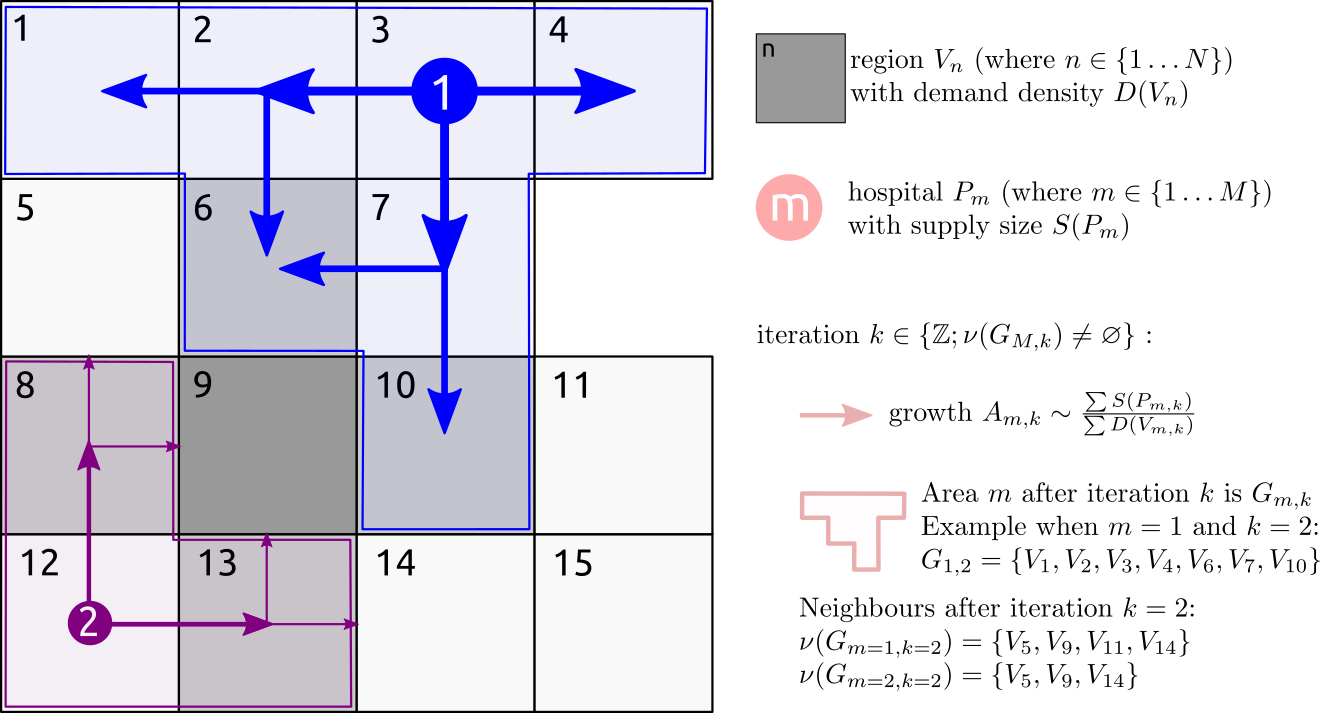
\includegraphics{FIG1_example.png} 
%   \caption{Schematic illustration of the proposed label propagation algorithm. The association of a hospital with a 
% region propagates from the hospital location (P) into the different regions (V) at a rate depending on the hospital 
% capacity S(P) and the population of the region, D(V), at each round of the iteration (k) until there are no more 
% neighbours to propagate a label to. The direction of spread is determined by the geographical neighbourhood of each 
% region V.}
%   \label{fig:one}
% \end{figure*}

Our goal is to divide the graph \(G\) into \(M\) labelled sub-graphs \(G_m\) such that the sub-graphs are connected, and 
that neighbouring sub-graphs have similar bed availability per unit population (\(\frac{\sum S_m}{\sum D_m}\)). We do 
this by assigning a score for each combination of region and hospital, which is initially zero. For every iteration of 
the algorithm this score is incremented in any unlabelled region that neighbours a region that has been labelled 
(i.e.~assigned to a specific hospital). The score is increased by a small amount determined by the ratio of supply 
(hospital beds) available, and demand (population to be served) in the regions assigned to that hospital. Thus labels 
propagate more quickly from points with a high capacity, through regions with a low population than vice-versa. The 
first label to propagate to a given area, and for which the score is above a threshold is defined as the ``supplier'' 
for that area, which is labelled as such. This ensures that each region is served by only one hospital.

\begin{algorithm*}%[H]
\setstretch{1.0}
\SetAlgoLined
\SetKwInOut{Input}{Input}
\SetKwInOut{Output}{Output}
\SetKwComment{Comment}{\--- }{}
\Input{$V_N$ - the $N$ regions of demand as a set of geographical polygons}
\Input{$D(V_n)$ - the density of demand in any given region as a function of the region $V_n$}
\Input{$P_M$ - a set of $M$ labelled suppliers as a set of geographical points}
\Input{$S(P_m)$ - the capacity of supply at any given supply point as a function of the supplier $P_m$}
\Input{$C_{growth}$ - a rate constant defining rate of label propagation}
\Output{$G_M$ - $M$ labelled subgraphs of graph $G$, relating to the catchment areas of suppliers $P_M$}
\BlankLine
\Comment{define $G$ as the graph consisting of geographical regions $V_N$, connected by edges, $E_N$, given by their 
geographical neighbours $\nu(V_N)$:}
$E_N \gets \nu(V_N)$\;
$G \gets (V_N, E_N)$\;
\Comment{define $V_M$ and $V^{new}_{M,0}$ as the geographic regions of $G$ serviced by points $P_M$, and $G_{M,0}$ as a 
set of labelled sub-graphs (also initially consisting solely of the vertices $V_M$):}
$V_M \gets G \cap P_M$\;
$V^{new}_{M,0} \gets V_M$;
$G_{M,0} \gets V_M$\;
\Comment{define the initial unlabelled set of vertices:}
$U_0 \gets \neg V_{M}$\;
\Comment{define the initial un-labelled neighbours of labelled sub-graphs, $G_M$:}
$U_{M,0} \gets \nu(V_M)$\;
\Comment{define an accumulated growth score for each un-labelled neighbour $U_{M,0}$ of each $G_{M,0}$:}
$A_{U_{M,0}} \gets 0$\;
\BlankLine
$k \gets 0$\;
\Comment{execute the loop while there are still unlabelled vertices and there exist some unlabelled neighbours of 
labelled vertices}
\While{$|U_k| > 0$ and $|U_{M,k}| > 0$} {
  $k \gets k+1$\;
  \BlankLine
  \Comment{define the un-labelled vertices as the set of $V$ not contained in any of $G_{M,k-1}$:}
  $U_k \gets \neg G_{M,k-1}$\;
  \Comment{define the un-labelled neighbours of $G_{M,k-1}$ as $U_{M,k}$ as the previously unlabelled neighbours and 
the neighbours of the most recently labelled neighbours $V^{new}_{M,k-1}$:}
  $U_{M,k} \gets U_{M,k-1} \cup (U_k \cap \nu(V^{new}_{M,k-1}))$\;
  \Comment{define the reserve capacity, $R_M$, to supply existing labelled, $G_{M,k-1}$,  and un-labelled neighbours 
$U_{M,k}$, as:}
  $R_M \gets \frac{S(P_M)}{D(U_{M,k} \cup G_{M,k-1})}$\;
  \Comment{for unlabelled areas only, update the accumulated growth score, $A_{U_{M,k}}$, with the normalised rank of 
the reserve capacity and multiplied by a constant $C_{growth} > 1$ representing the speed at which the accumulated 
growth score increases in all areas:}
  $R_{M,k} \gets R_m \{m \in U_{M,k}\}$\;
  $A_{U_{M,k}} \gets A_{U_{M,k-1}} + C_{growth} \times \text{rank}(R_{M,k})/|R_{M,k}|$\;
  \Comment{for all the un-labelled vertices, select the label $M$, with the highest score, and if the accumulated score 
has reached the threshold of 1, incorporate it into the labelled sub-graph, $G_{M,k-1}$:}
  $A^{max}_{U_k} = \text{max}(A_{U_{m,k}},m \in M)$\;
  $V^{new}_{M,k} \gets U_{M,k} \in \{A^{max}_{U_k} > 1\}$\;
  $G_{M,k} \gets G_{M,k-1} \cup V^{new}_{M,k}$\;
  $U_{M,k+1} \gets U_{M,k} \cap \neg V^{new}_{M,k}$\;
}
\Return{$G_{M,k}$}
\caption{A weighted label propagation algorithm for matching geographical supply to demand}
\end{algorithm*} 


\subsection*{Qualitative testing data}

The algorithm requires firstly an estimate of demand, for this we used population counts, secondly a geographical 
network and thirdly an estimate of supply, in this case hospital capacity data. 

For Great Britain there are detailed estimates of the population at granular geographic detail (lower super output area 
- LSOA) available from the Office of National Statistics (ONS) for England and Wales, and population estimates by Data 
Zone (DZ) are provided by the National Records Service (NRS) in Scotland 
\cite{PopulationEstimatesOffice,teamNationalRecordsScotland2013}. These population estimates are available by single 
year of age for each area. These are combined to create a single figure for the adult population of each small 
geographic area. 

Each geographical area is associated with a boundary files for lower super output areas and data zone from the 2011 
census, which are provided by the ONS and NRS \cite{OpenGeographyPortal,spatialdata.gov.scotDataZoneBoundaries2020}.

To estimate the capacity of hospitals we used a range of primary sources (described in the supplementary materials) to 
manually compile a list of NHS and independent hospital sites. When not provided in the primary sources, we identified 
their geographical locations from their postcode, and we estimated bed numbers from both a combination of published NHS 
statistics and from daily COVID-19 situation reports from early April 2020, provided by the NHS. The situation reports 
detailed both available beds at this point in time but also gave an indication of maximum surge capacity for high 
dependency beds. These data were manually curated and are indicative of the state of the NHS at maximal readiness. Bed 
state estimates for independent hospital providers were also available through the situation reports.

In Northern Ireland, population estimates were not available at a similar geographical resolution as the ONS and NRS 
sources, and we are unaware of any publicly available hospital capacity estimates. They were therefore not included in 
this analysis.

The detail of the original data sources we used is presented in the supplementary material, not all of which are 
publicly available. The algorithm is implemented as an R package \texttt{arear} (available from
\url{https://terminological.github.io/arear/}), which also contains both the manually curated hospital capacity and 
data pertaining derived demographics data described here. 

\subsection*{Validation}

There is no ground truth for the catchment areas for hospitals in the NHS during the COVID-19 pandemic. The rationale 
for original development of this algorithm was to make an estimate in absence of any activity data, in the early stages 
of the pandemic. Since then activity data has become available and this allows us to validate the label propagation 
approach to the activity based approach.

The activity based mapping takes the form of a many-to-many probabilistic mapping between lower tier local authority 
districts (LTLA) and NHS Acute Trusts in England derived from Secondary Uses Service (SUS) health-care data for England 
\cite{meakinNHSTrustLevel2021}. We create equivalent probabilistic associations between the coarse grained LTLA and NHS 
trusts by generating a fine grained lower super output area (LSOA) catchment area for NHS trusts using the label 
propagation algorithm, and the demographic and bed capacity estimates described above. This is aggregated to coarse 
grained local authority districts using mapping files provided by the ONS 
\cite{officeofnationalstatisticsLowerLayerSuper}, weighted by LSOA population size \cite{PopulationEstimatesOffice} 
(Source: Office for National Statistics licensed under the Open Government Licence v.3.0). This equivalent mapping 
based on the label propagation algorithm is compared to the activity based mapping graphically. To determine the degree 
of agreement between approaches the expected number of admissions to each NHS trust from each LTLA was estimated using 
each method. These were compared to each other using the intra-class correlation coefficient 
\cite{bartkoIntraclassCorrelationCoefficient1966,fisherStatisticalMethodsResearch1992} using a mean-of-raters, 
absolute-agreement, two-way random-effects model \cite{kooGuidelineSelectingReporting2016}, as implemented in the R 
package \texttt{irr} \cite{gamer2012package}. 

Secondly we obtain the coarse location (partial UK postcode, also known as outcode) from a list of intensive care 
patients admitted between 20th October 2000 and 16th March 2021 from the CHESS data set \cite{SGSSCHESSData}, which is 
an anonymised patient level hospital admission data set. We use outcode boundary shapes \cite{OpenDoorLogistics}, LSOA 
demographic estimates, and an areal interpolation \cite{prenerArealArealWeighted2020} to generate an estimate of 
demographics for each outcode. Using this outcode based regional population estimate, outcode boundary shapes, and the 
manually curated high dependency unit capacity estimates we calculate an outcode based catchment area estimate from 
which we are able to predict the NHS trust each patient was admitted to based on their outcode, which we compare to the 
observed NHS trust from the CHESS data. For this comparison we calculate both the multinomial accuracy, and for each 
NHS trust, the one-versus-all binomial accuracy as follows:

\[
\text{accuracy} = \frac{1}{|X|} \sum_{k \in G} \sum_{g_{obs}(x) = k} I \left(g_{pred}(x) = g_{obs}(x)\right)
\] 

where \(X\) is the set of observations, \(G\) is the set of NHS trusts, \(g_{pred}\) and \(g_{obs}\) are the predicted 
and observed classes respectively and \(I\) is the indicator function which returns \(1\) if the predicted match 
observed and \(0\) otherwise.

For the activity based approach we assign each patient to a LTLA by virtue of the geographical location of the centroid 
of their outcode shape and then determine the most probable NHS trust associated with that LTLA. This forms a prediction 
of the NHS trust based on the patient's outcode, which we can compare to the observed NHS trust in the same manner as 
above.

\section*{Results}

\subsection*{Qualitative testing results}

The results presented in this section qualitatively test the algorithm to determine whether it is producing catchment 
area regions that are geographically contiguous, aligned with existing demographic boundaries, and respect coarse 
geographical boundaries such as large rivers. The catchment areas should also produce estimates that minimise 
differences in the level of service provision from area to area, and we expect the overall regional variation of supply 
versus demand to be locally smooth. Figure ~\ref{fig:two} shows a catchment area based on individual hospitals that 
offered high dependency beds during April 2020, and a regional demand based on population estimates of adults in lower 
super output areas. The resulting set of catchment areas presented in panel A and C behave as desired in terms of the 
geographical properties. They also produce a fairly uniform density of high dependency bed provision per capita 
population, from region to region, as seen in panel B. In areas where there are high densities of hospitals such as 
London where the algorithm, by design, cannot propagate from centrally located hospitals past more peripheral 
hospitals, leading to small numbers of areas with high provision per head of population. This is discussed further 
below.

% \begin{figure*}[h!]
%   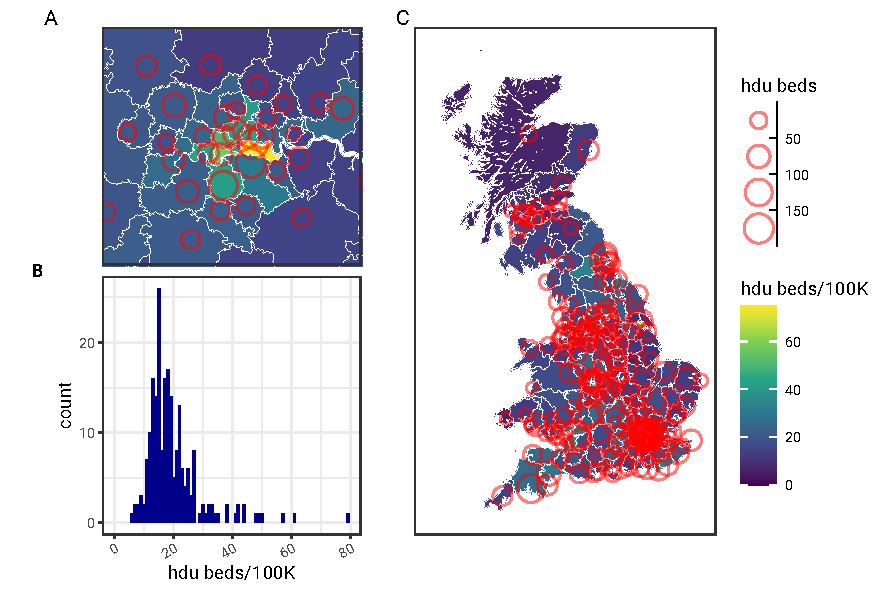
\includegraphics{FIG2_HDU_UK_example}
%   \caption{Panels A and C show a LSOA based catchment area map estimated from the high dependency bed state in Great 
% Britain in early April 2020, with catchment area boundaries shown in white. Red circles are NHS hospital sites with size 
% scaled to high dependency bed capacity. Map source: Office for National Statistics licensed under the Open Government 
% Licence v.3.0, Contains OS data © Crown copyright and database right 2020. Panel B shows the distribution of high 
% dependency beds per 100K population for each of the catchment areas defined by the algorithm.}
%   \label{fig:two}
% \end{figure*}


Further qualitative investigation of the properties of the algorithm are shown in Figure ~\ref{fig:three} where we see 
more regional detail of the same algorithm applied this time to general hospital beds rather than high dependency beds. 
Panel A shows the boundaries of the estimated catchment areas in white against the population density of a small area 
of the South West of England containing three hospitals (Plymouth, Torbay and the Royal Devon and Exeter hospitals). We 
can see in this example the extent of the catchment area to the South of Torbay is defined by the Dart river estuary, 
thus respecting topological constraints. 

Figure ~\ref{fig:three} panel B shows details about the progression of the algorithm from one iteration to the next, as 
labels propagate from each of the hospitals into the surrounding areas until encountering another catchment area. As we 
expect from the design the algorithm is seen to spread from hospital sites quickly through areas of low population 
(panel A), such as the countryside surrounding Plymouth in the bottom left, and more slowly through areas of higher 
population such as the areas surrounding Torbay in the middle right. 

% \begin{figure*}[h!]
%   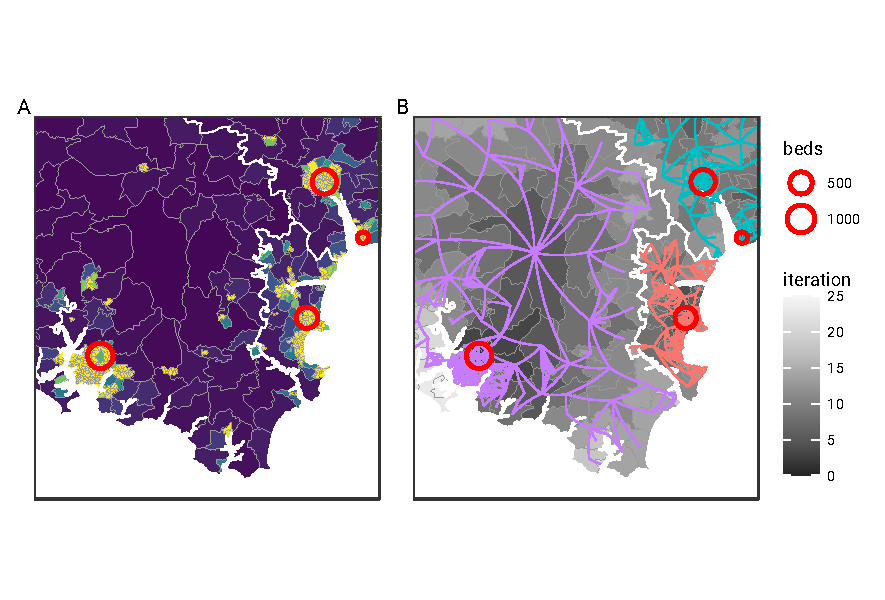
\includegraphics{FIG3_HDU_Acute_SW_example}
%   \caption{Detail LSOA based catchment area map for NHS trusts estimated from the general hospital bed states in Great 
% Britain in early April 2020. Red circles are NHS hospital sites. In panel A the fill represents a relative measure of 
% regional population density, with yellow areas being high density in and around cities. In Panel B the same areas are 
% shown but this time the fill shows the iteration number at which the algorithm labelled a specific area, and the 
% propagation of the algorithm by arrows. Map source: Office for National Statistics licensed under the Open Government 
% Licence v.3.0, Contains OS data © Crown copyright and database right 2020}
%   \label{fig:three}
% \end{figure*}

\subsection*{Validation}

In comparing the label propagation mapping to the activity based mapping we see that the proportions of any given LTLA 
that are assigned to any given trust are similar between the two methods Figure ~\ref{fig:four}, panel A) with a clear 
trend to agreement. The major differences are seen in the extremes where, for example, in the top left of panel A, the 
activity based approach may predict that no patients are observed in a given hospital from a given LTLA, whereas the 
label propagation approach predicts the opposite. Panel B shows the same relationship but this time scaled by the 
population size in each area, and this shows that the impact of differences between predictions seen in panel A is in 
areas with smaller populations and is therefore attenuated. Calculation of the intra-class correlation coefficient 
between the predicted number of cases from each method gives excellent agreement between the two methods, with a value 
of \dataInterRater{} using a mean-of-raters, absolute-agreement, two-way random-effects 
model \cite{kooGuidelineSelectingReporting2016}.

% \begin{figure*}[h!]
%   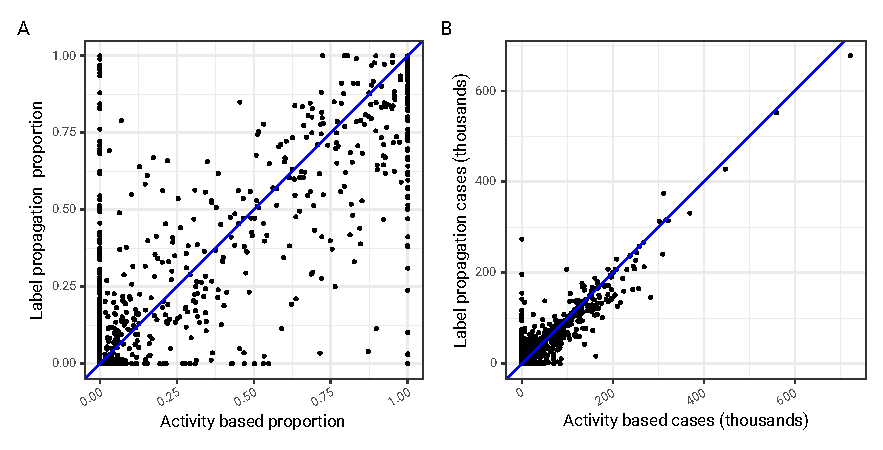
\includegraphics{FIG4_prob_comparison_agreement}
%   \caption{Classification agreement between activity based approach and label propagation algorithm. Each point is a 
% unique combination of lower tier local authority and NHS trust and in panel A the proportion of the LTLA assigned to 
% that trust is plotted for the activity based algorithm on the x-axis and the label propagation algorithm on the y-axis. 
% In panel B the total number of cases assigned to each trust is plotted when the population size for the area is 
% considered. The blue line represents perfect agreement.}
%   \label{fig:four}
% \end{figure*}

In Figure ~\ref{fig:five} we compare observed admissions to intensive treatment units (ITU) to predictions made by the 
label propagation algorithm and the activity based approach. As there are \dataNumItus{} trusts under consideration 
which form a large number of distractors for each prediction, a low value for the multinomial accuracy could be 
expected. The overall accuracy of both methods is comparable at \dataOverallAccuracy{}. The distribution of the 
binomial one-versus-all accuracy in the histogram shows that the prediction performance is better for some trusts than 
others, and that the accuracy of the activity based approach has greater variability than that of the label propagation 
approach. Across the whole country exact agreement between the observed location of hospital admission and the predicted 
location of hospital admission based on the label propagation catchment area was seen in \dataCorrect{} out of 
\dataTotal{} cases, and the Matthew's correlation coefficient was \dataMcc{}. 

% \begin{figure*}[h!]
%   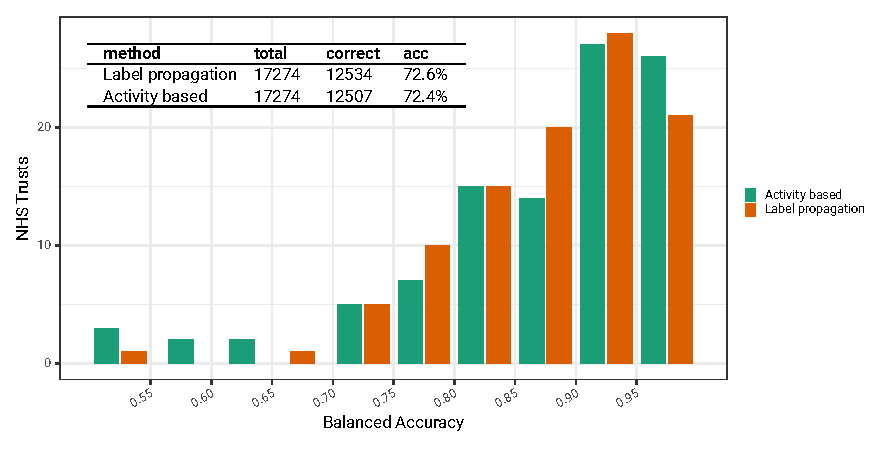
\includegraphics{FIG5_sari_accuracy_comparison} 
%   \caption{Accuracy measures for the predictions of activity based and label propagation approaches based on UK postcode 
% outcodes, and a subset of observed NHS trust of intensive care admissions in England between 20th October 2000 and 16th 
% March 2021. The histogram shows the distribution of the balanced accuracy for each NHS trust in a one-vs-all binomial 
% evaluation, and the inset table shows the overall accuracy from the multinomial evaluation, along with the raw counts of 
% overall evaluations and correct predictions for each method}
%   \label{fig:five}
% \end{figure*}

The ten NHS Trusts that have the highest number of ITU patients that the label propagation algorithm predicted to be 
admitted elsewhere, represent \dataTopMisclass{} (\dataTopMisclassPercent{}) of the total 
misclassifications. On inspection the majority of these 10 hospitals are major tertiary referral intensive care units, 
or specialist centres and are in the top quintile of NHS trusts by ITU bed capacity. This could be explained if 
severely ill patients may end up in specialist centres rather than their closest hospital for treatment, or that in the 
event of a large surge in cases, patients may overflow from smaller to larger intensive care units. Both of these 
could lead to misclassification of these patients by the label propagation algorithm.

\section*{Discussion}

We have presented an algorithm for rapidly estimating hospital catchment areas for use when activity data is not 
available. We demonstrate how the output responds to the different capacities of the different levels of care provided 
(e.g. high dependency versus general hospital beds). We present catchment areas calculated using population size as 
demand, and total hospital beds as supply. This algorithm may be useful for longer term strategic planning, but was 
conceptualised as part of an acute response to COVID-19 outbreak. In this case we can use the different parameters for 
demand, for example local COVID-19 infection prevalence, and different parameters for supply, for example availability 
to staffed hospital beds. Our approach is novel in that it allows adaptation of local service provision to predictions 
of disease prevalence from epidemiological models of COVID-19 and real time bed states provided by NHS trusts. This 
allows us to model the degree of elasticity in the system to absorb localised shocks, caused by regional outbreaks, it 
helps us to develop a better concept of when services are being at risk of becoming overwhelmed, and allow routing of 
new admissions away from overloaded hospitals.

Bench-marking our algorithm against activity based approaches produced good to excellent agreement and application to 
both methods to real world patient admission data produces a very similar result. The finding that naive application of 
our algorithm to real world patient admission classifies only \dataAcc{} correctly is explained by two things, firstly 
accuracy at boundaries decreases as the number of boundaries increases \cite{arcayaAreaVariationsHealth2012} and 
secondly the fact that many of the top 10 misclassified trusts are major tertiary referral centres, which may take 
patients from distant regions for specialist care. This suggests that our constraint that catchment areas should be non 
overlapping is not borne out in reality for these cases. 

Overlapping catchment areas could be modelled by multiple layers of non-overlapping catchment areas. When we consider 
the provision of intensive care services in the UK during COVID-19, we propose there are at least 3 layers of hospital 
service provision: there is a local service, which provides care for patients from nearby. A subset of hospitals 
additionally provide a regional, or tertiary referral, service layer which takes sicker patients from neighbouring 
hospitals in larger areas. The final layer is a crisis overflow layer provided by the NHS Nightingale field hospitals 
\cite{CoronavirusNightingaleHospital2020}. Each of these layers may be considered to have somewhat independent 
catchment areas, a phenomenon that has been observed in variable uptake of spinal services in Switzerland 
\cite{scheuterUnwarrantedRegionalVariation2018}. We propose that dividing the larger hospitals into local and regional 
services and considering the tertiary referral network as a second layer, with its own larger catchment area would 
improve the performance of the algorithm against real activity data. In such a layered model of catchment areas there is 
interplay between local layer demand for hospital beds and capacity for regional tertiary care provision, which will 
dynamically affect the "catchment area" for regional tertiary care provision, potentially on a day to day basis. In 
previous work we looked at the opportunities for balancing the load between different hospitals 
\cite{lacasaFlexibleMethodOptimising2020} when transferring COVID-19 patients away from overloaded areas, however moving 
unwell patients between hospitals is ideally minimised. With this algorithm we enable the dynamic re-specification of 
local service catchment areas and hospital tertiary referral networks, based on evolving demand. Coupled with flexible 
load sharing has interesting potential to model or influence patient admissions around the whole hospital network.

Hospital capacity is difficult to accurately estimate. During this work we encountered many of the uncertainties that 
influence capacity. The ability of a hospital to provide a bed to a patient depends on a multitude of factors, 
including staff availability, which may vary during the different stages of the pandemic. The ability of hospitals to 
absorb large numbers of emergency patients by re-configuring their service provision (e.g cancelling routine 
operations) and providing overflow or "surge" high dependency capacity for short periods of time makes putting a single 
number on hospital capacity difficult. The ability to recalculate catchment areas based on changing assumptions around 
capacity is a strength of our approach, and in the future could be used to analyse the impact of introducing new 
capacity into the hospital system. One further limitation to note is that the algorithm does not consider travel time 
between regions which may increase both as the geographical size increases but also as the population density increases 
due to traffic and form a barrier to patients accessing services. Adding a travel time penalty to the rate of label 
spread into the model is possible given some estimate of the ease of transport within and between regions, and this is 
an area of future work.

Our approach is limited to situations where the relationship between hospitals and the population is mostly driven by 
population density and geography. This may be more relevant to national health services such as the NHS, and less 
relevant to more commercial hospital systems in which there are many different factors influencing the patients decision 
as to what hospital they attend. However, even within these systems our approach may be useful for service planning in 
larger hospital groups, when we consider capacity planning for specific services such as radiology.

There are opportunities to extend our algorithm. The general approach of label propagation in networks has been more 
widely studied and newer approaches described 
\cite{xieCommunityDetectionUsing2011,gregoryFindingOverlappingCommunities2010,sunDetectingOverlappingCommunities2015} 
which allow overlapping communities. This may address some of the issues described above. These are appealing and a 
possible avenue for future extension of the algorithm. There persists however an open question about whether the 
overlapping nature of hospital service provision observed in activity data is not really a reflection of patient 
choice, but actually the result of subtly different services, or different levels of service, being provided by 
different hospitals to different catchment areas. Thus a specialist cancer hospital close to a specialist paediatric 
hospital will have geographically overlapping catchment areas, but in reality these hospitals are not providing the same 
service to the same population. This line of argument suggests that the concept of a single overlapping hospital 
catchment area is also an over-simplification, and when we take into account the heterogeneity of different services 
offered by a hospital, we propose that a hospital's overall catchment area may be well modelled by a collection of 
non-overlapping catchment layers.

\section*{Conclusions}

This label propagation algorithm for estimating hospital catchment areas is a pragmatic solution to determining 
geographical and demographic subsets of the population when there is no previous activity data available. It suits 
situations where the level of service provision and demand on the hospital system is dynamic, as has been the case in 
the COVID-19 pandemic. The algorithm is simple and satisfies the major criteria we set out in the introduction, in that 
it provides a mapping from low level geographic regions which provide contiguous and realistic subdivisions of 
geographies relating to a single hospital or to a group of hospitals. The areas are determined by the capacity of the 
hospital and the size of local population, and are approximately equal in terms of local supply (e.g. beds) and demand 
(e.g. patients) at boundaries.

The algorithm depends solely on data reflecting supply and geographical demand for a service, and as such is quite 
generic and potentially more widely applicable outside of healthcare. Although we have discussed catchment areas in 
terms of the capacity of hospital beds, and demand of local populations, there is nothing to prevent us defining 
capacity in any other way - a heuristic on staffing levels may be appropriate, or in different contexts, availability 
of medical imaging devices. Likewise, demand may be refined to reflect sub-populations at risk of disease, or may even 
be the output of a predictive model. As such our approach is applicable to a wide variety of problems.

%%%%%%%%%%%%%%%%%%%%%%%%%%%%%%%%%%%%%%%%%%%%%%
%%                                          %%
%% Backmatter begins here                   %%
%%                                          %%
%%%%%%%%%%%%%%%%%%%%%%%%%%%%%%%%%%%%%%%%%%%%%%

\begin{backmatter}

\section*{Acknowledgements}%% if any
Many thanks to TJ McKinley at the University of
Exeter, for feedback on an early draft of the paper and testing of the
implementation of the algorithm.

\section*{Funding}%% if any
RC and KTA gratefully acknowledge the financial support
of the EPSRC via grant EP/N014391/1. KTA gratefully acknowledge the
financial support of The Alan Turing Institute under the EPSRC grant
EP/N510129/1 and EP/T017856/1. RC is supported by NHS England, Global
Digital Exemplar programme and the MRC (MC/PC/19067). LL acknowledges
the financial support of the EPSRC via Early Career Fellowship
EP/P01660X/1. GJG is supported by an ESRC postdoctoral fellowship
ES/T009101/1.

\section*{Availability of data and materials}%% if any
The majority of data and a reference implementation of the  algorithm 
is implemented as an R package \texttt{arear} (available from
\url{https://terminological.github.io/arear/}). The CHESS data that support
part of the validation findings of this study are available from Public Health England but
due to the fact the data is at single individual level, albeit anonymised,
restrictions apply to the availability of these data. These which were used
under license for the current study, and so are not publicly available.
This validation data are however available from the authors upon reasonable request and
with permission of Public Health England. 

\section*{Ethics approval and consent to participate}%% if any
Data on cases were
obtained from the COVID-19 Hospitalisation in England Surveillance
System (CHESS) data set that collects detailed data on patients infected
with COVID-19. These data contain confidential information, with public
data deposition non-permissible for socioeconomic reasons. The CHESS
data resides with the National Health Service (www.nhs.gov.uk). Data
from the CHESS database were supplied after anonymisation under strict
data protection protocols agreed between the University of Exeter and
Public Health England. The ethics of the use of these data for these
purposes was agreed by Public Health England with the Government's
SPI-M(O) / SAGE committees.

\section*{Competing interests}
The authors declare no financial
relationships with any organisations that might have an interest in the
submitted work in the previous three years, no other relationships or
activities that could appear to have influenced the submitted work.

\section*{Consent for publication}%% if any
The author is the copyright holder and consents to publication

\section*{Authors' contributions}
All authors discussed the concept of the
article and RC wrote the initial draft. KTA, LL, GG commented and made
revisions. All authors read and approved the final manuscript. RC is the
guarantor.

%%%%%%%%%%%%%%%%%%%%%%%%%%%%%%%%%%%%%%%%%%%%%%%%%%%%%%%%%%%%%
%%                  The Bibliography                       %%
%%                                                         %%
%%  Bmc_mathpys.bst  will be used to                       %%
%%  create a .BBL file for submission.                     %%
%%  After submission of the .TEX file,                     %%
%%  you will be prompted to submit your .BBL file.         %%
%%                                                         %%
%%                                                         %%
%%  Note that the displayed Bibliography will not          %%
%%  necessarily be rendered by Latex exactly as specified  %%
%%  in the online Instructions for Authors.                %%
%%                                                         %%
%%%%%%%%%%%%%%%%%%%%%%%%%%%%%%%%%%%%%%%%%%%%%%%%%%%%%%%%%%%%%

% if your bibliography is in bibtex format, use those commands:
\bibliographystyle{bmc-mathphys} % Style BST file (bmc-mathphys, vancouver, spbasic).
\bibliography{catchment-areas}      % Bibliography file (usually '*.bib' )
% for author-year bibliography (bmc-mathphys or spbasic)
% a) write to bib file (bmc-mathphys only)
% @settings{label, options="nameyear"}
% b) uncomment next line
%\nocite{label}

% or include bibliography directly:
% \begin{thebibliography}
% \bibitem{b1}
% \end{thebibliography}

%%%%%%%%%%%%%%%%%%%%%%%%%%%%%%%%%%%
%%                               %%
%% Figures                       %%
%%                               %%
%% NB: this is for captions and  %%
%% Titles. All graphics must be  %%
%% submitted separately and NOT  %%
%% included in the Tex document  %%
%%                               %%
%%%%%%%%%%%%%%%%%%%%%%%%%%%%%%%%%%%

%%
%% Do not use \listoffigures as most will included as separate files

\section*{Figures}

\begin{figure*}[h!]
  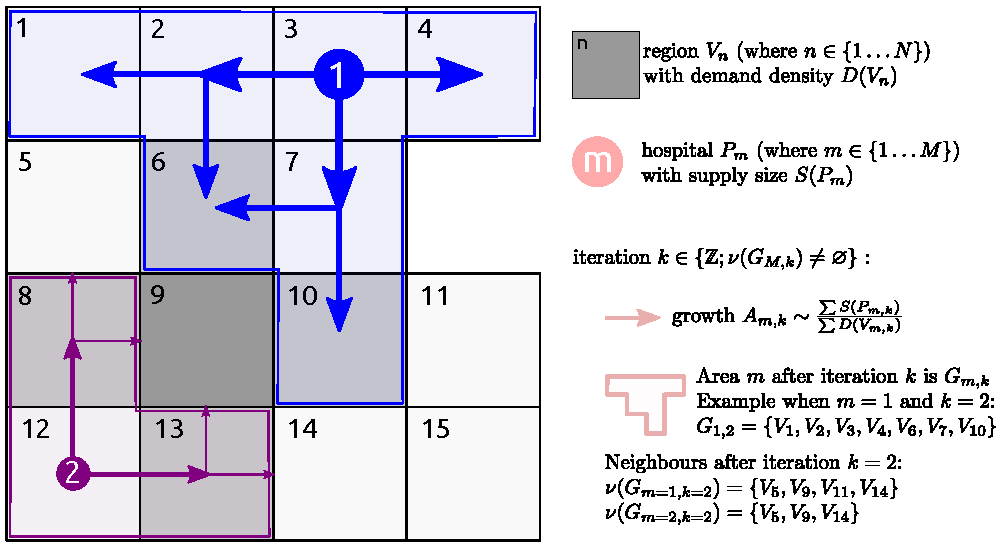
\includegraphics{FIG1_example} 
  \caption{Schematic illustration of the proposed label propagation algorithm. The association of a hospital with a 
region propagates from the hospital location (P) into the different regions (V) at a rate depending on the hospital 
capacity S(P) and the population of the region, D(V), at each round of the iteration (k) until there are no more 
neighbours to propagate a label to. The direction of spread is determined by the geographical neighbourhood of each 
region V.}
  \label{fig:one}
\end{figure*}

\begin{figure*}[h!]
  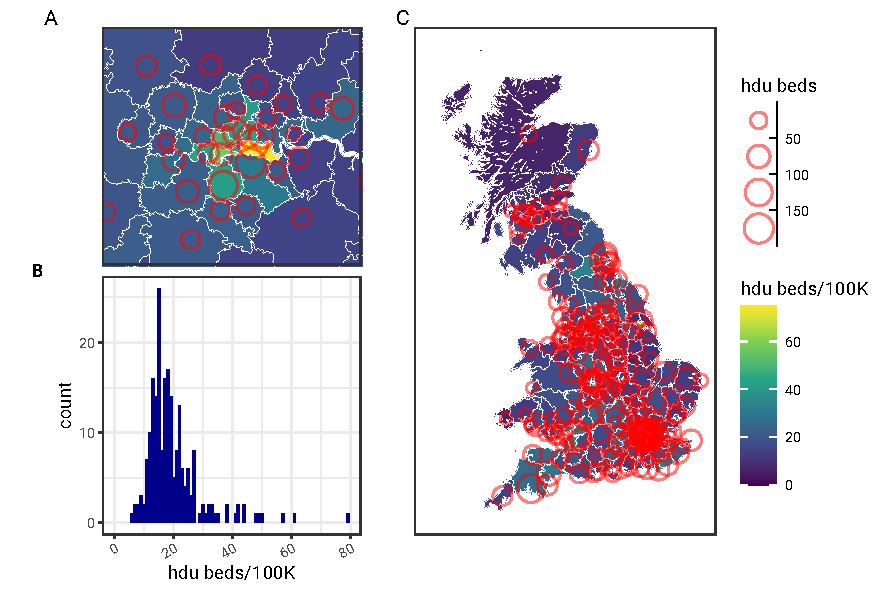
\includegraphics{FIG2_HDU_UK_example}
  \caption{Panels A and C show a LSOA based catchment area map estimated from the high dependency bed state in Great 
Britain in early April 2020, with catchment area boundaries shown in white. Red circles are NHS hospital sites with 
size 
scaled to high dependency bed capacity. Map source: Office for National Statistics licensed under the Open Government 
Licence v.3.0, Contains OS data © Crown copyright and database right 2020. Panel B shows the distribution of high 
dependency beds per 100K population for each of the catchment areas defined by the algorithm.}
  \label{fig:two}
\end{figure*}

\begin{figure*}[h!]
  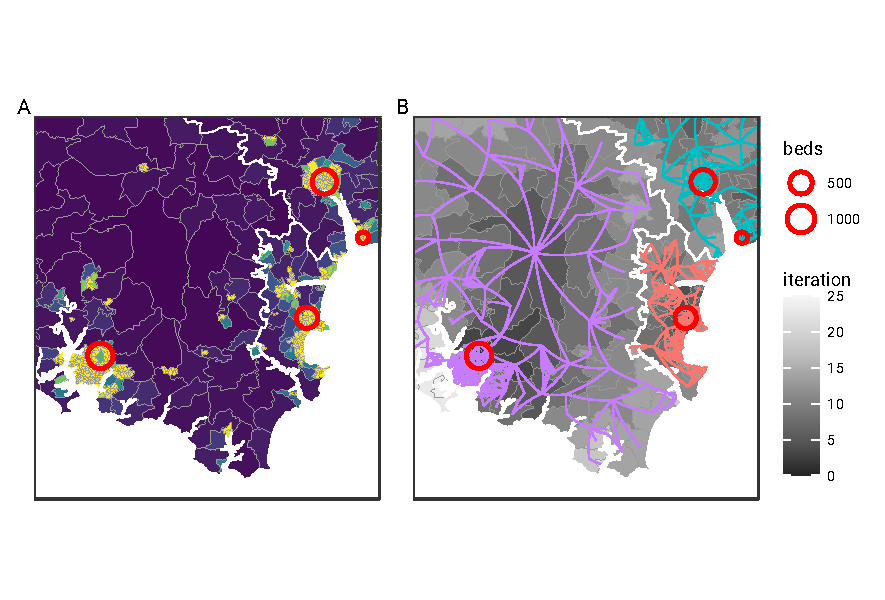
\includegraphics{FIG3_HDU_Acute_SW_example}
  \caption{Detail LSOA based catchment area map for NHS trusts estimated from the general hospital bed states in Great 
Britain in early April 2020. Red circles are NHS hospital sites. In panel A the fill represents a relative measure of 
regional population density, with yellow areas being high density in and around cities. In Panel B the same areas are 
shown but this time the fill shows the iteration number at which the algorithm labelled a specific area, and the 
propagation of the algorithm by arrows. Map source: Office for National Statistics licensed under the Open Government 
Licence v.3.0, Contains OS data © Crown copyright and database right 2020}
  \label{fig:three}
\end{figure*}

\begin{figure*}[h!]
  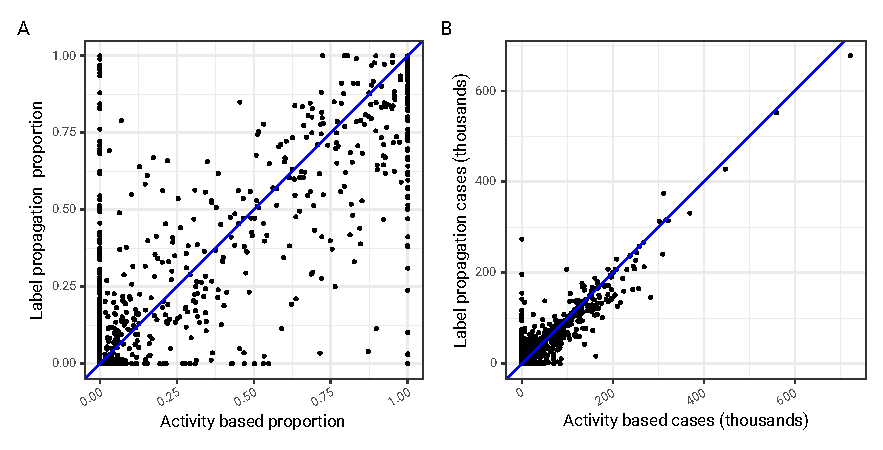
\includegraphics{FIG4_prob_comparison_agreement}
  \caption{Classification agreement between activity based approach and label propagation algorithm. Each point is a 
unique combination of lower tier local authority and NHS trust and in panel A the proportion of the LTLA assigned to 
that trust is plotted for the activity based algorithm on the x-axis and the label propagation algorithm on the y-axis. 
In panel B the total number of cases assigned to each trust is plotted when the population size for the area is 
considered. The blue line represents perfect agreement.}
  \label{fig:four}
\end{figure*}

\begin{figure*}[h!]
  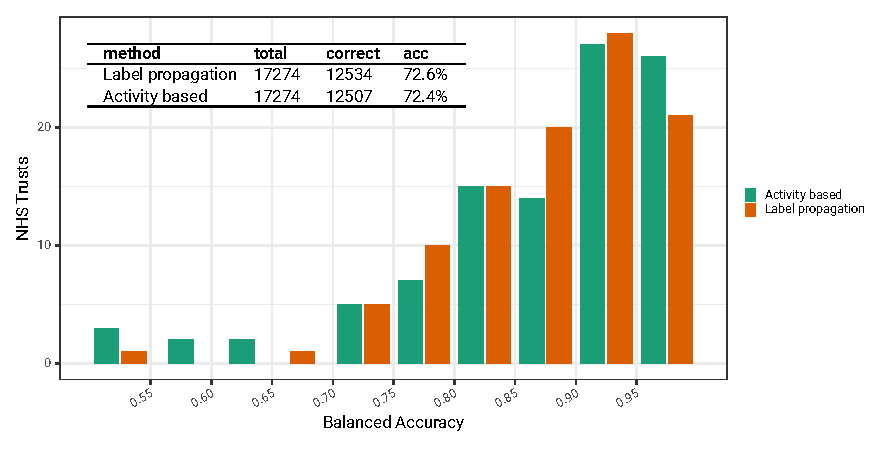
\includegraphics{FIG5_sari_accuracy_comparison} 
  \caption{Accuracy measures for the predictions of activity based and label propagation approaches based on UK 
postcode 
outcodes, and a subset of observed NHS trust of intensive care admissions in England between 20th October 2000 and 16th 
March 2021. The histogram shows the distribution of the balanced accuracy for each NHS trust in a one-vs-all binomial 
evaluation, and the inset table shows the overall accuracy from the multinomial evaluation, along with the raw counts 
of 
overall evaluations and correct predictions for each method}
  \label{fig:five}
\end{figure*}

%%%%%%%%%%%%%%%%%%%%%%%%%%%%%%%%%%%
%%                               %%
%% Additional Files              %%
%%                               %%
%%%%%%%%%%%%%%%%%%%%%%%%%%%%%%%%%%%

\section*{Additional Files}
  \subsection*{Additional file 1 --- Supplementary material - algorithmic hospital catchment area estimation using 
label propagation}
    Sources of hospital capacity data, population estimates,  and some additional visualisations.

  \subsection*{Additional file 2 --- Supplementary data - surge capacity estimates}
    A curated data set of estimated acute and ITU bed capacity in the NHS and private hospitals at the start of the 
pandemic, in England, Wales, and Scotland.

\end{backmatter}
\end{document}
